\documentclass[aspectratio=169]{beamer}
\usetheme[
    section page = progressbar,
    progressbar = foot,
    background = light
]{metropolis}

\newcounter{notes}
\setcounter{notes}{0}

% define general format and includes for all assignments
\documentclass[10pt, largemargins]{../homework}
\usepackage{geometry}

% import req basic packages
\usepackage[dvipsnames]{xcolor}
\usepackage[tracking=true]{microtype}
\usepackage{amsmath, amssymb}
\usepackage{hyperref}
\usepackage{subcaption}
\usepackage{graphicx}
\usepackage{ifthen}
\usepackage[utf8]{inputenc}
\usepackage{braket}


% set font
\usepackage[T1]{fontenc}
\usepackage{baskervillef}
\usepackage[varqu,varl,var0]{inconsolata}
\usepackage[scale=.95,type1]{cabin}
\usepackage[baskerville,vvarbb]{newtxmath}
\usepackage[cal=boondoxo]{mathalfa}


% reviews and notes
\ifthenelse{\value{draft} > 0}
{
  \newcommand{\parth}[1]{\textcolor{OliveGreen}{$\left[\textnormal{Parth: #1}\right]$}}
  \newcommand{\sahas}[1]{\textcolor{TealBlue}{$\left[\textnormal{Sahas: #1}\right]$}}
  \newcommand{\sankalp}[1]{\textcolor{WildStrawberry}{$\left[\textnormal{Sankalp: #1}\right]$}}
}
{
  \newcommand{\parth}[1]{}
  \newcommand{\sahas}[1]{}
  \newcommand{\sankalp}[1]{}
}

% homework class and document settings
\newcommand{\hwname}{Parth Sastry, Sahas Kamat, Sankalp Gambhir}
\newcommand{\hwemail}{\texttt{180260026, 30, 32}}
\newcommand{\hwtype}{Assignment}
\newcommand{\hwnum}{0} % default number
\newcommand{\hwclass}{PH423}
\newcommand{\hwlecture}{} % unused, but needed
\newcommand{\hwsection}{} % unused, but needed

\title{Equivalence Between Systems Stronger than Resolution \\
{\small M.L. Bonet, Jordi Levy}}
\author{Sankalp Gambhir}

\begin{document}
    \frame{\titlepage}
    %
    \section{Resolution...?}
    \begin{frame}
        \frametitle{Resolution}
        It is an inference rule. \pause

            \[\begin{prooftree}
                \hypo{x \lor A}
                \hypo{\lnot x \lor B}
                \infer2{\pause A \lor B}
            \end{prooftree}
            \quad \textit{CUT}
            \]

        \pause This is the Resolution inference rule, done! \pause However this
        is not quite the form we need it in. This rule is incomplete in the case
        we try to apply it to MaxSAT instead\pause, so we would like to modify
        it to fit our needs. 
    \end{frame}
    \begin{frame}
        \frametitle{MaxSAT Resolution}
        The goal is to find a maximal set of simultaneously satisfiable clauses
        by cardinality, or alternately, the minimum number of unsatisfiable
        clauses for any assignment. \pause The main issue with MaxSAT is that we
        cannot have our inference rules changing the number of unsatisfiable
        clauses. This is how we define a \emph{sound} inference rule in MaxSAT.
        \notes{Unfortunately, solving the Max-SATproblem forφis, in general,
        notequivalentto solving it forφ′; i.e., the number of unsatisfiedclauses
        inφandφ′is not the same for every truth assignment. Therefore, if we
        want to compute anoptimal solution, we cannot apply unit propagation as
        in SATsolvers.}

        As for Resolution --

        \begin{multicols}{2}
            \[\begin{prooftree}[center, separation=2.5em]
                \hypo{x \lor A}
                \hypo{\lnot x \lor B}
                \infer2{A \lor B}
            \end{prooftree}\]

            \pause
            \columnbreak

            \[\begin{prooftree}[center, separation=2.5em]
                \hypo{x \lor A & \lnot x \lor B}
                \infer1{\pause A \lor B \pause \quad x \lor A \lor \overline{B} \pause \quad \lnot x \lor \overline{A} \lor B}
            \end{prooftree}\]

        \end{multicols}

        \notes{The exact form of this is not too important for our purposes here.}
    \end{frame}
    %
    \section{What's stronger? \\ {\tiny I hope not more than 5 minutes have passed}}
    \begin{frame}
        \frametitle{Circular Proofs}
        
        \notes{Consider for a second, a water tank. If we draw 5 lines of water from
        it, it's gonna empty out real quick. Some of the pipes go around the
        place, then back into the tank. Starting with an empty tank, you get...
        nothing. However, if overall, the number of pipes leaving the tank was
        smaller than the number of pipes coming in, we might just have a full
        tank on our hands. }  

        % insert image!!
        \centering
        \scalebox{1}{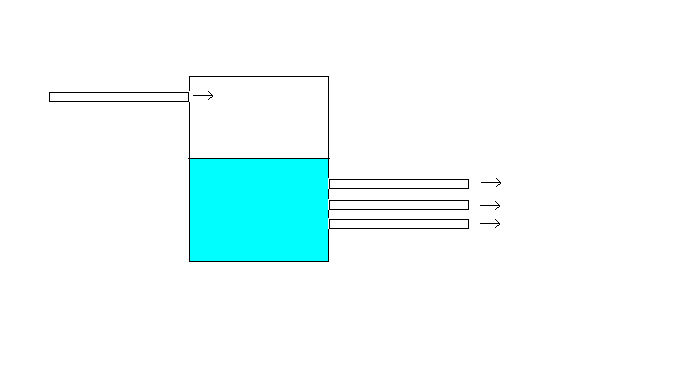
\includegraphics[width=\textwidth]{fig/water.png}}
    \end{frame}
    \begin{frame}
        \frametitle{Circular Proofs}

        \begin{multicols}{2}
            \centering
            \begin{tikzpicture}[
            roundnode/.style={circle, draw=red!60, fill=red!15, very thick, minimum size=7mm},
            squarednode/.style={rectangle, draw=blue!60, fill=blue!5, very thick, minimum size=5mm},
            ]
            %Nodes
            \node[roundnode]      (ax)                              {$x \lor A$};
            \node[squarednode]    (split)         [below=of ax] {SPLIT};
            \node[roundnode]      (x)           [below=of split] {$x$};
            \node[roundnode]      (xx)          [right=of split] {$x \lor \lnot x$};
            \node[squarednode]    (cut)         [below=of xx] {CUT};
            \node[roundnode]      (ax2)         [right=of cut] {$x \lor A$};
    
            %Lines
            \draw[->] (ax) -- (cut);
            \draw[->] (x)  to [out=150,in=210]  (split);
            \draw[->] (split) -- (x);
            \draw[->] (split) -- (xx);
            \draw[->] (xx) -- (cut);
            \draw[->] (cut) -- (ax2);
            \end{tikzpicture}

            \notes{Rather blood tanks now that I've written the colors the wrong way around}
            
            \pause
            \columnbreak
            \justify

            SPLIT and CUT have \emph{flows}. These flows allow us to calculate
            the balance on each formula node. \pause For each formula in the
            system, we must have a non-negative balance\pause, and for our goal
            in particular, we would like the tank to be filled and not just
            passing water, per the analogy, so we want a positive balance.
            \cite{atserias2019circular}

        \end{multicols}

    \end{frame}
    %
    \begin{frame}
        \frametitle{Weighted Proofs}
        
        \notes{In MaxSAT, replace instances of a clause $A$ by a pair $(A, n)$ with n
        being the number of times it occurs. Negative weights can be used to
        signify clauses that haven't been proved.}

        \[A, A, \ldots , A \rightarrow (A, n)\]
        
        \pause Weighted MaxSAT in particular is equivalent to the normal MaxSAT.
        \notes{Because you can just interchange the occurences and numbers.}
        \pause \\Where does n lie? \notes{What is the domain of n? Positive? Non
        Negative? All integers?} \pause What could $n = -2$ mean? \notes{You
        might see this is suspiciously similar to our analogy earlier. So we try
        to look at them together.}
    
    \end{frame}
    \section{Equivalence and Dual Rail Proofs\\
    {\tiny As much as I'd like to think I have 5 more minutes...}}
    \begin{frame}
        \frametitle{Equivalence}
        \notes{I hope I have convinced you by way of analogy that the two
        discussed systems are indeed equivalent. Resolution seems somewhat
        foreign to this discussion, but the rest of the focus is on equivalence
        of these systems under arbitrary inference rules and what it means for
        the restriction to resolution and MaxSAT in particular.}

        \notes{I will give an outline of the proof.}

        So take the balance we discussed for circular proofs, and start with
        those as weights for your weighted proof. \notes{We can freely sever
        certain edges and create a total ordering of the nodes.} Traversing the
        nodes, each of the inference rules, having a \emph{flow} associated to
        it, can be seen as combining and modifying the weights.
        \cite{bonet2020equivalence} \notes{Proof seems quite intuitive, it's
        just hard to show that it does indeed satisfy all the conditions for a
        weighted proof.} 
    \end{frame}
    \begin{frame}
        \frametitle{Equivalence}
        \notes{The other direction is simpler, especially now that we have
        explicitly established a correspondence between the two ideas.} 
        \pause

        For the other direction, start with nodes corresponding to the
        hypothesis, and for each step of the weighted proof, introduce nodes for
        the inference rules, with appropriate flow values inferred from the
        weights used. The main issue is proving, again, that the final weights
        satisfy our conditions.
    \end{frame}
    \begin{frame}
        \frametitle{Equivalence}
        \notes{So why would you care? Circular proofs are annoying enough,
        analogies and everything. Everything is equivalent anyway. Circular
        proofs give us intuitive representations of proof ideas, and provide
        intuition for extensions of weighted proofs by being able to access the
        more general ideas of flow networks in graph theory.} Why do I care?
        \pause Graphs!

        \pause Infact, the actual proof of equivalence relies on introducing
        terms of the form $(A, n), (A, -n)$. \pause This inherently circular ideology
        allows us to simplify our proofs by introducing clauses before they're
        available, making promises for their arrival. \pause All's fine, \emph{as long
        as we keep our promises.}
    \end{frame}

    \begin{frame}
        \frametitle{Dual Rail Disbelief of Making it this Far}
    
        The basic idea behind Dual Rail Proofs is simple, treat literals $x$ and
        $\lnot x$ as different variables. \pause This creates several issues in
        the case of SAT as we know, unless your clauses are in certain forms.
        \pause Here, manipulating the weights allows us to (somewhat) simplify
        that issue, while helping our cause too. \notes{We would need to
        explicitly derive empty clauses to obtain unsat.}
    
    \end{frame}

    \begin{frame}
        \frametitle{Dual-Rail Equivalent systems }
    
        No general version of this proof is given. The discussion is limited to
        Dual Rail MaxSAT (with resolution) and what we need to add to
        circular/weighted proofs to obtain equivalence. \pause Turns out, not
        too bad. \pause Allowing 0-SPLITs, i.e. +n, -n clauses from nothing,
        instead of the usual SPLIT, makes it equivalent.
    
    \end{frame}

    \begin{frame}{References}
        \bibliographystyle{amsalpha}
        \bibliography{ref.bib}
    \end{frame}
\end{document}